\documentclass[a4paper,12pt]{report}


\usepackage[utf8]{inputenc}		% Accents, etc
\usepackage[frenchb]{babel} 		% Francais
\usepackage[T1]{fontenc}			% Encodage de police (césure, accents)
\usepackage{lmodern,textcomp}	% Polices 'Latin Modern' plutôt que 'Computer Modern super'

\usepackage[pdftex]{graphicx}			% Graphiques (images, ...)
\usepackage{amsmath,amssymb}		% Equations
\usepackage[pdftex]{hyperref}	% Lien table des matières

\usepackage{titlesec}			% Chapitres
\titleformat{\chapter}[hang]{\bf\huge}{\thechapter}{2pc}{}

% Symbole euro €
\usepackage{eurosym}

% Floating figures
\usepackage{wrapfig}

% Subfigures
\usepackage{subfig}

% Marges du document
\usepackage{geometry}
\geometry{top=2cm, bottom=2cm, left=25mm, right=25mm}

%
\usepackage{rotating}

% Taille des sous-titres
%\usepackage{titlesec}
%\titleformat{\subsection}{\small\bfseries}{\thesection}{1em}{}

% Page de titre du document
\title{Projets de groupe \\ Rapport de reformulation}
%\author{J. \bsc{Fanguede}, F. \bsc{Castellane}, G. \bsc{Mahieux}, F. \bsc{Tavares}}
\author{\bsc{J. Fanguede} \and \bsc{F. Castellane} \and \bsc{G. Mahieux} \and \bsc{F. Tavares}  }
\date{Février 2012}

% Réglages des métadata du PDF
\hypersetup{
pdftitle={Rapport de reformulation},
pdfauthor={J. Fanguede, F. Castellane, G. Mahieux, F. Tavares},
pdfsubject={Projets de groupe 2012},
pdfkeywords={Phelma, Projet, Grenoble, INP, Flyport, OpenPicus}
}
% Ligne horizontale
\newcommand{\HRule}{\rule{\linewidth}{0.5mm}}


% Début du document
\begin{document}

\begin{titlepage}
	\begin{center}
	
	% Upper part of the page
	
\includegraphics[width=0.25\textwidth]{images/smallphelma.png}\\[1.8cm]    

	\textsc{\LARGE Grenoble INP -- Phelma}\\[1.5cm]

	\textsc{\Large Projet de groupe}\\[0.5cm]


	% Title
	\HRule \\[0.4cm]
	{ \huge \bfseries Rapport de reformulation}\\[0.4cm]

	\HRule \\[1.5cm]

	% Author and supervisor
	\begin{minipage}{0.3\textwidth}
		\begin{flushleft} \large
			\emph{Groupe:}\\
			J. \textsc{Fanguede}, \\ F. \textsc{Castellane}, \\ G. \textsc{Mahieux}, \\ F. \textsc{Tavares}
		\end{flushleft}
	\end{minipage}
	\begin{minipage}{0.4\textwidth}
		\begin{flushright} \large
			\emph{Tuteur:} \\
			M. Sylvain \textsc{Huet}
		\end{flushright}
	\end{minipage}
	\vfill

% Bottom of the page
{\large \today}

\end{center}

\end{titlepage}

% Page de titre du document
%\maketitle

% Introduction
\chapter*{Introduction}
Les projets de groupe occupent une place importante dans le programme pédagogique de la première année à Phelma. Ils permettent à chacun de travailler en groupe sur une thématique choisie. En outre, ils offrent une première expérience de gestion et de réalisation de projet. 

Ce rapport a pour but de présenter le projet qui a été choisi, de clarifier ses objectifs et d’exposer les solutions techniques envisagées pour sa réalisation.

% Table des matières
\tableofcontents

% Début du document
\chapter{Présentation du projet}


	\section{Problématique et objectifs}
	Le sujet de projet que nous avons choisi est : «~voiture radio-commandée en Wi\nobreakdash-Fi~». L’objectif du projet est de concevoir le système de commande d’un modèle réduit de voiture, ceci incluant aussi bien l’électronique embarquée que le logiciel de contrôle à distance du véhicule.

Ce projet de robotique a principalement attiré notre attention du fait de sa multi-disciplinarité. En effet, la réalisation d’un tel système implique des compétences à la fois en électronique et en informatique. Or, nous partagions tous un intérêt prononcé pour l’informatique et la programmation.

Ce projet de réalisation d’une voiture radio-commandée en Wi-Fi peut surprendre au premier abord. En effet, une connexion Wi-Fi est plus compliquée à mettre en œuvre, donc plus chère et plus consommatrice qu’une liaison RF maître-escalve habituellement utilisée dans ce type de systèmes. Cependant, l’avantage du Wi-Fi est qu’il offre une couche d’abstraction logicielle de haut niveau permettant des communications à double sens entre le contrôleur et la machine à contrôler. C’est-à-dire qu’il est possible de faire remonter facilement des informations à partir de capteurs embarqués sur le véhicule.

C’est donc plus dans une optique de \emph{robot explorateur} que de \emph{jouet radio-commandé} qu’il faut comprendre la démarche que nous avons mené.


	\section{Cahier des charges fonctionnel}
	Le système réalisé devra comporter un certain nombre de fonctionnalités obligatoires à son bon fonctionnement. En particulier, pouvoir contrôler le véhicule d’une manière relativement fluide, offrir une interface de contrôle sur une plate-forme adaptée et disposer d’une autonomie d’au moins quelques minutes. Le cahier des charges fonctionnel est décrit figure~\ref{cdcf}.

Des améliorations pourront par la suite être apportées à l’ensemble afin d’améliorer ses performances et ses fonctionnalités. On pensera notamment, dans la continuité de la section précédente, à des capteurs divers, une caméra, etc. Ces fonctionnalités seront implémentées en fonction de l’avancement du projet et des accords de budget de l’administration.

\begin{figure}%[!h]
	\begin{enumerate}
		\item Voiture radio-commandée
		\begin{enumerate}
    			\item Système de connectivité sans-fil
				\begin{enumerate}
    					\item Norme Wi-Fi IEEE 802.11 B/G/N
    					\item Protocoles de communication standards (ex: TCP / IP)
  				\end{enumerate}
    			\item Être contrôlable par un protocole interne
				\begin{enumerate}
    					\item Syntaxe des commandes
  				\end{enumerate}
			\item Rouler à une vitesse satisfaisante
			\item Avoir une autonomie suffisante
    			\item Offrir un retour d’informations au client
				\begin{enumerate}
    					\item Niveau de batterie
					\item Capteurs de proximité
					\item Caméra vidéo
  				\end{enumerate}
  		\end{enumerate}

		\item Logiciel de télécommande
		\begin{enumerate}
    			\item Être implémentable facilement sur une grande variété de plates-formes
				\begin{enumerate}
    					\item Utilisation de protocoles de communication standards (voir 1.a.ii)
  				\end{enumerate}
    			\item Offrir une interface utilisateur conviviale et fonctionnelle
				\begin{enumerate}
    					\item Contrôles adaptés à la plate-forme (ordinateur, smartphone)
  				\end{enumerate}
			\item Pouvoir afficher certaines grandeurs en temps réel (voir 1)
  		\end{enumerate}
	\end{enumerate}

	\caption{Cahier des charges fonctionnel}
	\label{cdcf}
\end{figure}


	\section{Schéma fonctionnel}
	En accord avec le cahier des charges, la figure~\ref{schemafonctionnel} présente rapidement les différentes composantes de l’ensemble et leurs interactions. Celui-ci est composé de deux entités : la télécommande et le véhicule.

Sur la télécommande doit être chargé le logiciel de contrôle qui va être développé. Celui-ci permettra de contrôler le véhicule, de modifier ses réglages réseau et d’observer les signaux en provenance des capteurs. On privilégiera une plate-forme mobile ouverte du type Android.

La voiture devra disposer d’un module Wi-Fi et d’un micro-controlleur programmable, permettant de contrôler les moteurs et de lire les valeurs des capteurs embarqués. L’alimentation (batterie) devra pouvoir alimenter l’ensemble de l’électronique embarquée.

\begin{figure}%[!h]
	\begin{center}
		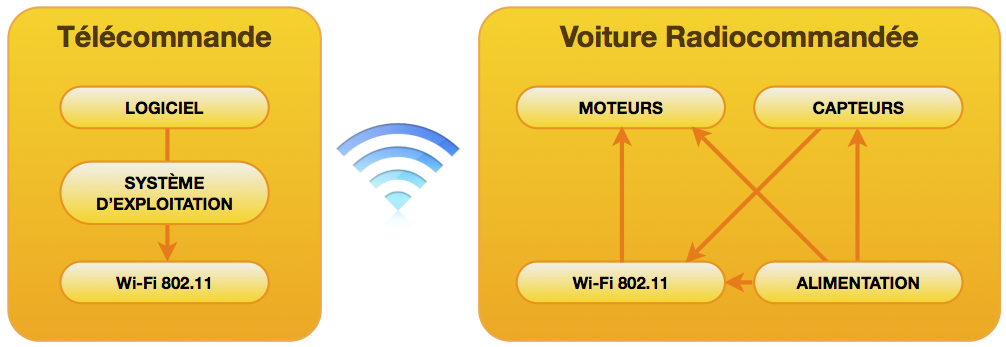
\includegraphics[scale=0.75]{images/schemafonctionnel.png}
	\end{center}
	\caption{Schéma fonctionnel du système} 
	\label{schemafonctionnel}
\end{figure}

	
	\section{Solutions techniques}
		Le pré-découpage du système, présenté précédemment, permet d’envisager des solutions techniques pour chacune de ses composantes.
		
		\subsection{Motorisation du véhicule}
		Nous avons décidé de nous focaliser plus sur l'aspect électronique du système que sur la mécanique de la voiture. En effet, nous disposions d'un modèle réduit 1/10\ieme{} motorisé sur lequel nous pourrions installer notre système. Cela nous donnera l'assurance que le moteur et la batterie sont bien dimensionnés et nous permettra de nous concentrer sur l'électronique embarquée et le logiciel de contrôle.
		
Le contrôle du moteur sera effectué par le module Wi-Fi via un pont en H. Le pont en H est un circuit simple permettant de séparer l'alimentation et le contrôle d'un moteur. Le pont devra être adapté au moteur utilisé, en termes de tension et de courant.

		\subsection{Module Wi-Fi embarqué}
		Pour pouvoir communiquer avec le monde extérieur, notre voiture doit comporter un module répondant aux exigences de la norme Wi-Fi. Quel élément pouvons-nous utiliser ?
			
			\paragraph{Single-board Computer}
			Une première solution envisageable est d’utiliser un single-board Computer (SBC) tel le \href{http://www.raspberrypi.org/}{Raspberry Pi} basé sur une distribution Linux. Pour pouvoir piloter la voiture, deux options s’offrent à nous : soit choisir un modèle avec Wi-Fi intégré, soit s’appuyer sur un \emph{dongle} USB Wi-Fi classique. Outre une installation et une utilisation relativement aisées, cette solution permet de brancher facilement un large éventail de périphériques en USB. Cependant, un tel dispositif reste relativement encombrant, gourmand en énergie et cher, des critères non négligeables dans un tel projet.
		
		\paragraph{Micro-contrôleur programmable}
		Une seconde possibilité est de s’appuyer sur un micro-contrôleur programmable. S’il existe une grande variété de produits de ce type sur le marché, le choix se restreint quand on prend en compte le fait que notre module doit pouvoir gérer une connexion Wi-Fi de lui-même. Un dispositif répond toutefois à nos exigences : le FlyPort Wi-Fi, fabriqué la société OpenPicus (\href{http://www.openpicus.com}{www.openpicus.com}).

Premier point positif, le langage de programmation utilisé nous est familier car il s’agit du C accompagné d'API de haut niveau. De plus, cette solution demeure moins encombrante, moins énergivore, mais également plus flexible qu'un SBC puisqu'il dispose d'une vingtaine d'entrées-sorties \emph{remappables} à la volée. En somme, elle est tout indiquée pour un système embarqué. L’ajout de périphériques sera en revanche plus délicat. Par ailleurs, ce produit a un coût relativement élevé (68€ HT) bien que la société OpenPicus ait la gentillesse de nous faire don d'un \emph{Starter Kit} pour notre projet.

\begin{figure}[!h]
  \centering
  \subfloat[Un SBC]{\label{fig:SBC}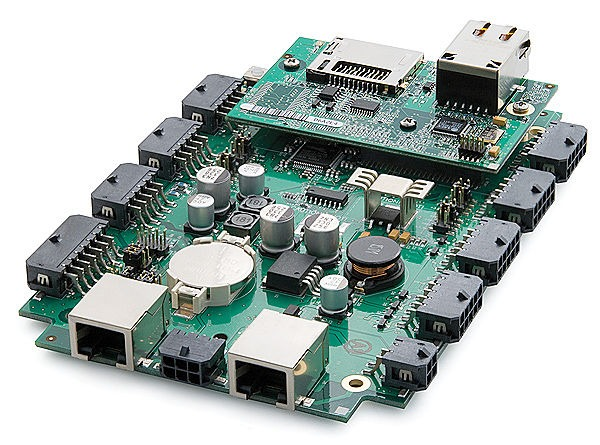
\includegraphics[width=0.22\textwidth]{images/SBC.png}}
  \hspace{20pt}
  \subfloat[Le module Flyport]{\label{fig:flyport}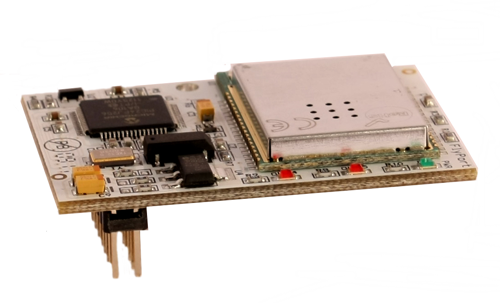
\includegraphics[width=0.3\textwidth]{images/flyport.png}}
  \caption{Solutions envisagées}
  \label{fig:animals}
\end{figure}

\bigskip
Après analyse des avantages et des défauts de chaque proposition, nous avons décidé de retenir le \emph{FlyPort} pour jouer le rôle du module Wi-Fi.

		\subsection{Télécommande}
		La télécommande sera programmée directement sur un système  disposant d’une interface Wi-Fi de haut niveau. De plus, celle-ci devra comporter une interface utilisateur de type graphique (GUI). Plusieurs plateformes sont retenues : les ordinateurs personnels et les smartphones. Il est important de préciser que les exigences de l’application de commande sont directement liées au support considéré. Nous allons les expliciter ci-dessous.
		
			\paragraph{Smartphone}
			Ici, la priorité est de réaliser une interface conviviale permettant à l’utilisateur un contrôle rapide et facile de la voiture. Un problème demeure : sur quel OS travailler ? On remarque qu’Android et iOS équipent plus de la moitié des terminaux mobiles. Toutefois, un développement pour iOS demeure assez contraignant : il nécessite notamment de posséder un Mac et un compte développeur payant. Le développement pour Android nécessite quant à lui l’utilisation du langage Java. Nous avons donc décidé de retenir la plateforme Android pour la version portative de la télécommande.
			
			\paragraph{Ordinateur personnel}
			Cette interface pourra présenter des fonctionnalités avancées, absentes de la version mobile. On pense notamment à un réglage des paramètres réseaux. Pour le développement, il nécessaire d’utiliser une bibliothèque graphique. Au vu de la variété des environnements de développement des personnes travaillant sur ce projet (PC/Mac/Linux), la solution doit être multi-plateforme, c'est-à-dire que le même code source devra pouvoir être compilé et exécuté sur toutes les machines. De plus, pour des raisons de coût, la licence doit être gratuite. Plusieurs solutions existent en la matière, les deux plus répandues étant Qt et WxWidget. Toutes les deux nécessitent d’utiliser le langage C++. Nous avons décidé de retenir Qt pour sa documentation plus large et sa plus grande communauté d’utilisateurs.
			
	\section{Besoins matériels et financiers}
	Le tableau ci dessous récapitule le matériel nécessaire à la réalisation du projet. certains composants sont en option car il ne sont utile qu’à la réalisation d’objectifs secondaires.
	
\begin{center}\scriptsize
	\begin{tabular}{|l|l|l|l|}
	\hline
	\texttt{} \footnotesize\bf{Désignation} & \footnotesize\bf{Origine} & \footnotesize\bf{Tarif (TTC)} & \footnotesize\bf{Notes} \\ \hline
	\texttt{} Module Wi-Fi OpenPicus Starter Kit  & Sponsoring OpenPicus & 81~€ & Livré \\ \hline
	\texttt{} Voiture RC & Matériel Personnel & 40~€ & Oui \\ \hline
	\texttt{} Servomoteur (Hitec HS-422) & Magasin Minatec & 11~€ & Retiré au magasin \\ \hline
	\texttt{} Pont en H intégré L298 & STMicroelectronics Samples & 8~€ & Livraison en cours \\ \hline
	\texttt{} Contrôleur Moteur DC (MC33926) & Roboshop.com & 21.56~€ + FDP & Demande de budget en cours \\ \hline
	\texttt{} Caméra &  & 50~€ & \emph{facultatif} \\ \hline
	\texttt{} Capteurs divers &  & 10~€ & \emph{facultatif} \\ \hline
	\end{tabular}
\end{center}

\chapter{Organisation et communication}


	\section{Charte de travail en équipe}
	
		\subsubsection{Répartition des rôles et des tâches}
		La gestion du groupe se fait de façon collégiale, et il a été fait le choix de ne pas désigner de chef de projet. Chacun des membres du groupe est responsable d'une partie du projet et devra faire preuve d'initiative afin de mener à bien son travail.
		
En ce qui concerne la répartition des tâches, celles-ci sont évaluées au début de chaque séance puis réparties entre les différents membres pour plus d'efficacité. Un petit bilan sera effectué en fin de séance et le carnet de bord mis à jour par chacun des membres après la séance.

Les tâches non techniques (rédaction de rapports, communication avec le tuteur, etc.) seront réparties de la manière la plus équitable possible.


		\subsubsection{Séances hebdomadaires}
		Les séances auront lieu a la fréquence d'une fois par semaine, le vendredi de 13h30 à 17h30 à Minatec, en salle M372.
		
		
		\subsubsection{Règles de vie}
		Les membres du groupe devront autant que possible respecter certaines règles, notamment :
		
		\begin{itemize}
			\item respecter les autres membres du groupe ;
			\item être présent au séances de projet ;
			\item respecter les horaires prévus ;
			\item respecter le planning des tâches.
		\end{itemize}
		
		\bigskip
		Quelques règles de sécurité devront également s'appliquer afin d'éviter tout accident :
		
		\begin{itemize}
			\item manipuler avec précaution le fer à souder ;
			\item toujours prévenir les autres membres du groupe avant de faire des manipulations dangereuses.
		\end{itemize}
		

		\subsubsection{Communication}
		Nous avons décidé de communiquer principalement par courrier électronique, en dehors des séances de projet. Chaque mail devra être adressé à tous les membres du groupe afin que chacun soit au courant des avancées des autres.
		
		De plus un service de partage de documents et de travail collaboratif à été mis en place (Google Documents). On y trouvera tous les documents importants concernant le projet. Notamment le carnet de bord, que chacun des membres pourra compléter selon ses souhaits.
	
		Un hébergement de projet à également été mis en place (Google Code). Il permet d’utiliser un logiciel de gestion des versions (SVN Subversion) ainsi qu'un \emph{wiki}. Tous les membres du groupe ont la possibilité de partager leur code et d'autres documents sur ce serveur. Le \emph{wiki} contiendra des informations sur les différentes parties du projet ainsi que des explications de certains codes.


	\section{Déroulement du projet}
	
	Le découpage du système et l'analyse des besoins nous a permis d'identifier un certain nombre de tâches à effectuer dans le cadre du projet. Celles-ci sont représentées sur le diagramme figure~\ref{wbs}
	
	\begin{figure}%[!h]
	\begin{center}
		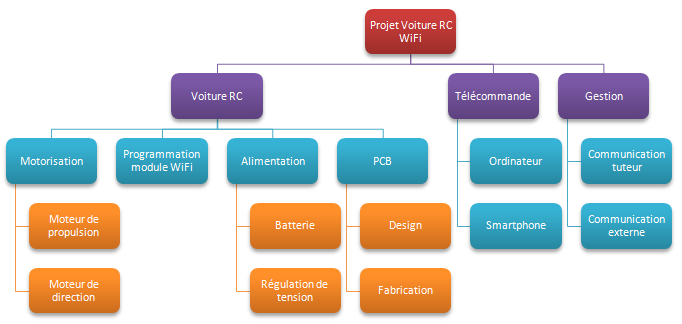
\includegraphics[scale=1.1]{images/wbs.png}
	\end{center}
	\caption{Diagramme WBS} 
	\label{wbs}
	\end{figure}
	
	Le diagramme de Gantt en annexe (figure~\ref{gantt}) présente le déroulement du projet et la répartition des tâches dans le temps. Il permet de voir les grandes phases successives du projet (analyse, conception du système, programmation, communication).
	
	
	\section{Communication externe}
	La société OpenPICUS nous a offert le \emph{starter kit} Flyport à la condition que nous acceptions de communiquer sur notre projet avec la communauté d'utilisateurs OpenPICUS. Ce \emph{sponsoring} leur permet de faire la publicité de leur produit auprès des établissements d'enseignement supérieur, de faire grandir la communauté d'utilisateurs et de créer une vitrine de projets démontrant les capacités du produit.
	
	Le site que nous avons mis en place sur Google Code est donc en accès libre à l'adresse : \href{http://code.google.com/p/flyport-wifi-rc-car/}{http://code.google.com/p/flyport-wifi-rc-car/}. On y trouvera les choix techniques que nous avons fait, les programmes réalisés et divers documents complémentaires.
	
\begin{sidewaysfigure}
\centering
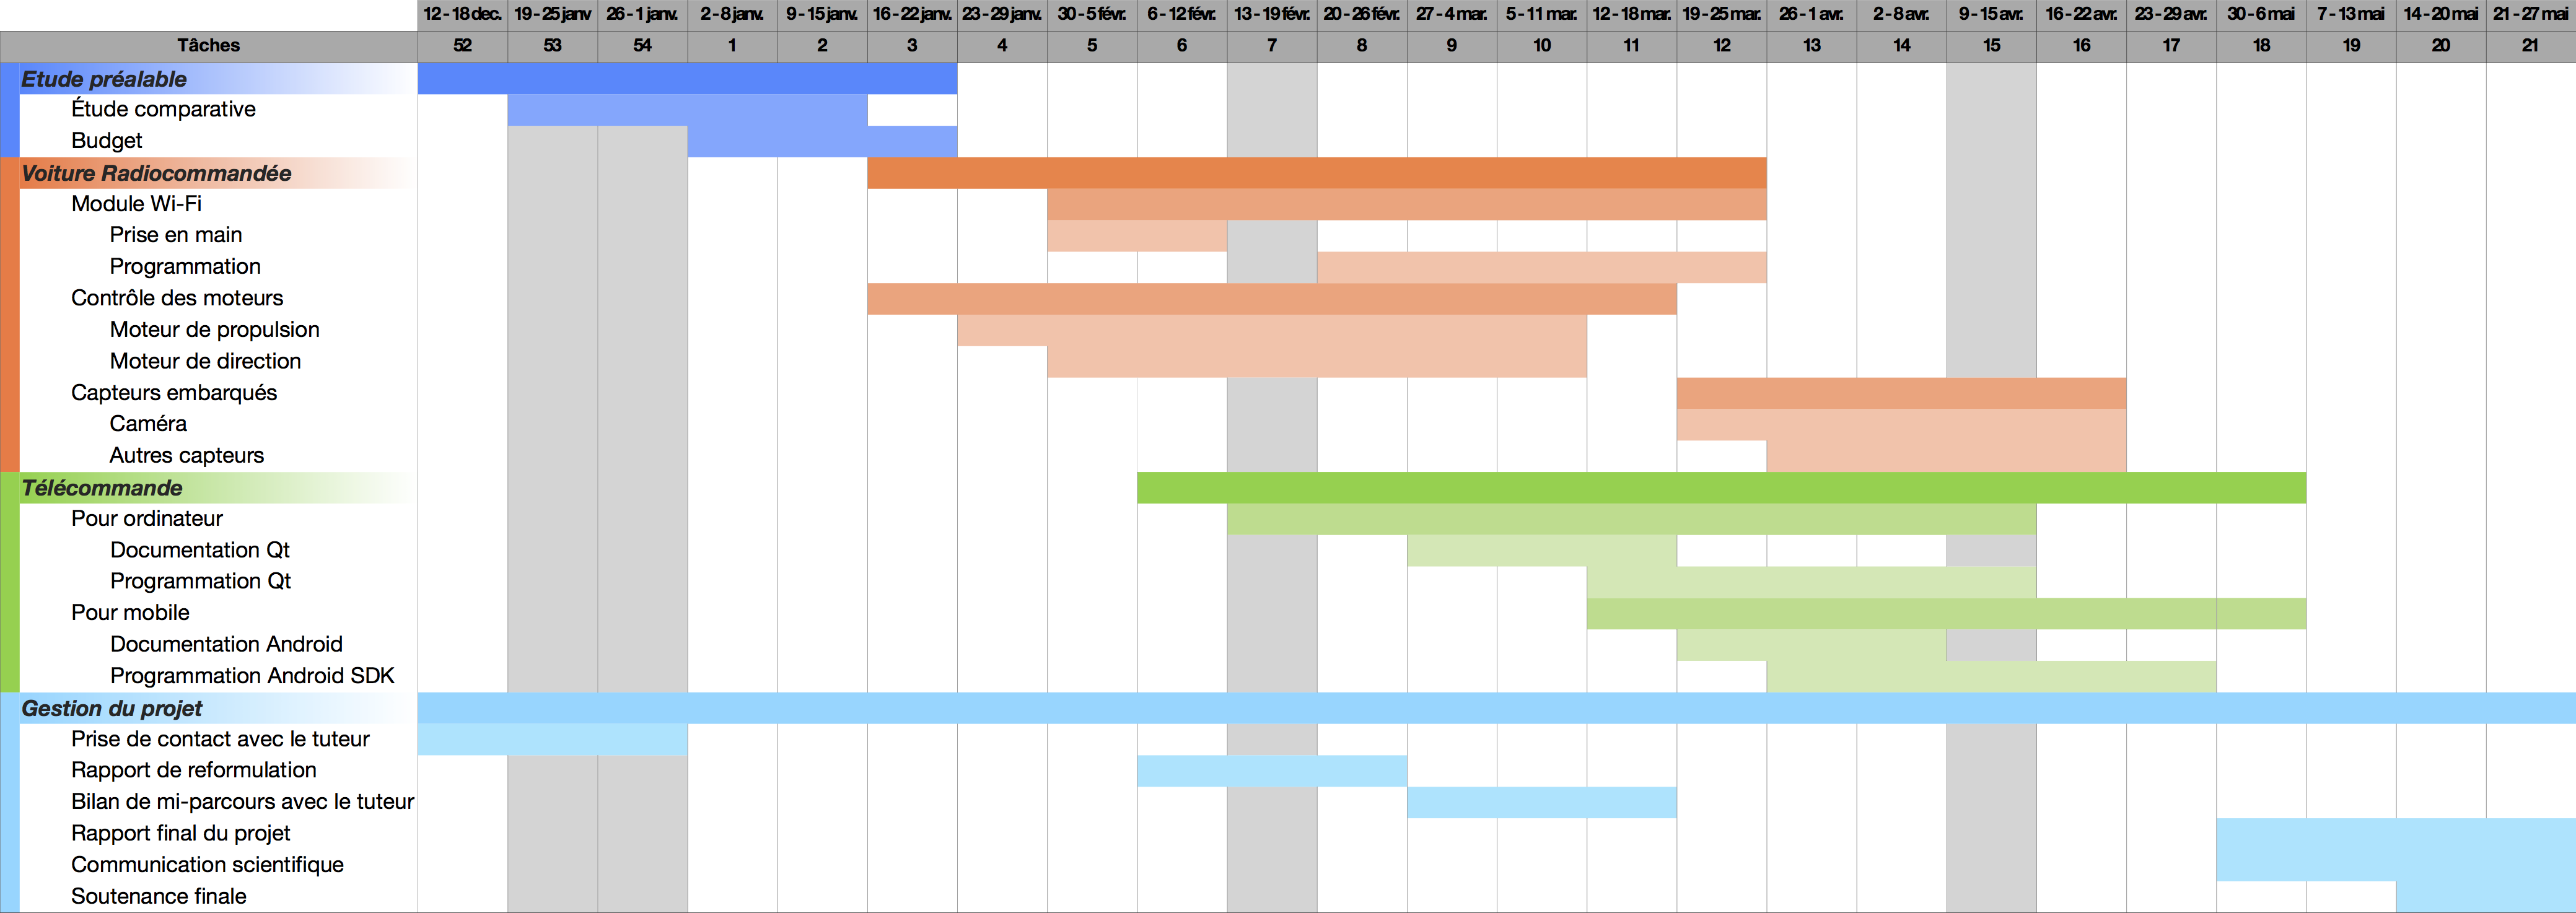
\includegraphics[scale=0.35]{images/gantt.png}
\caption{Diagramme de GANTT}
\label{gantt}
\end{sidewaysfigure}

	%\centering
	%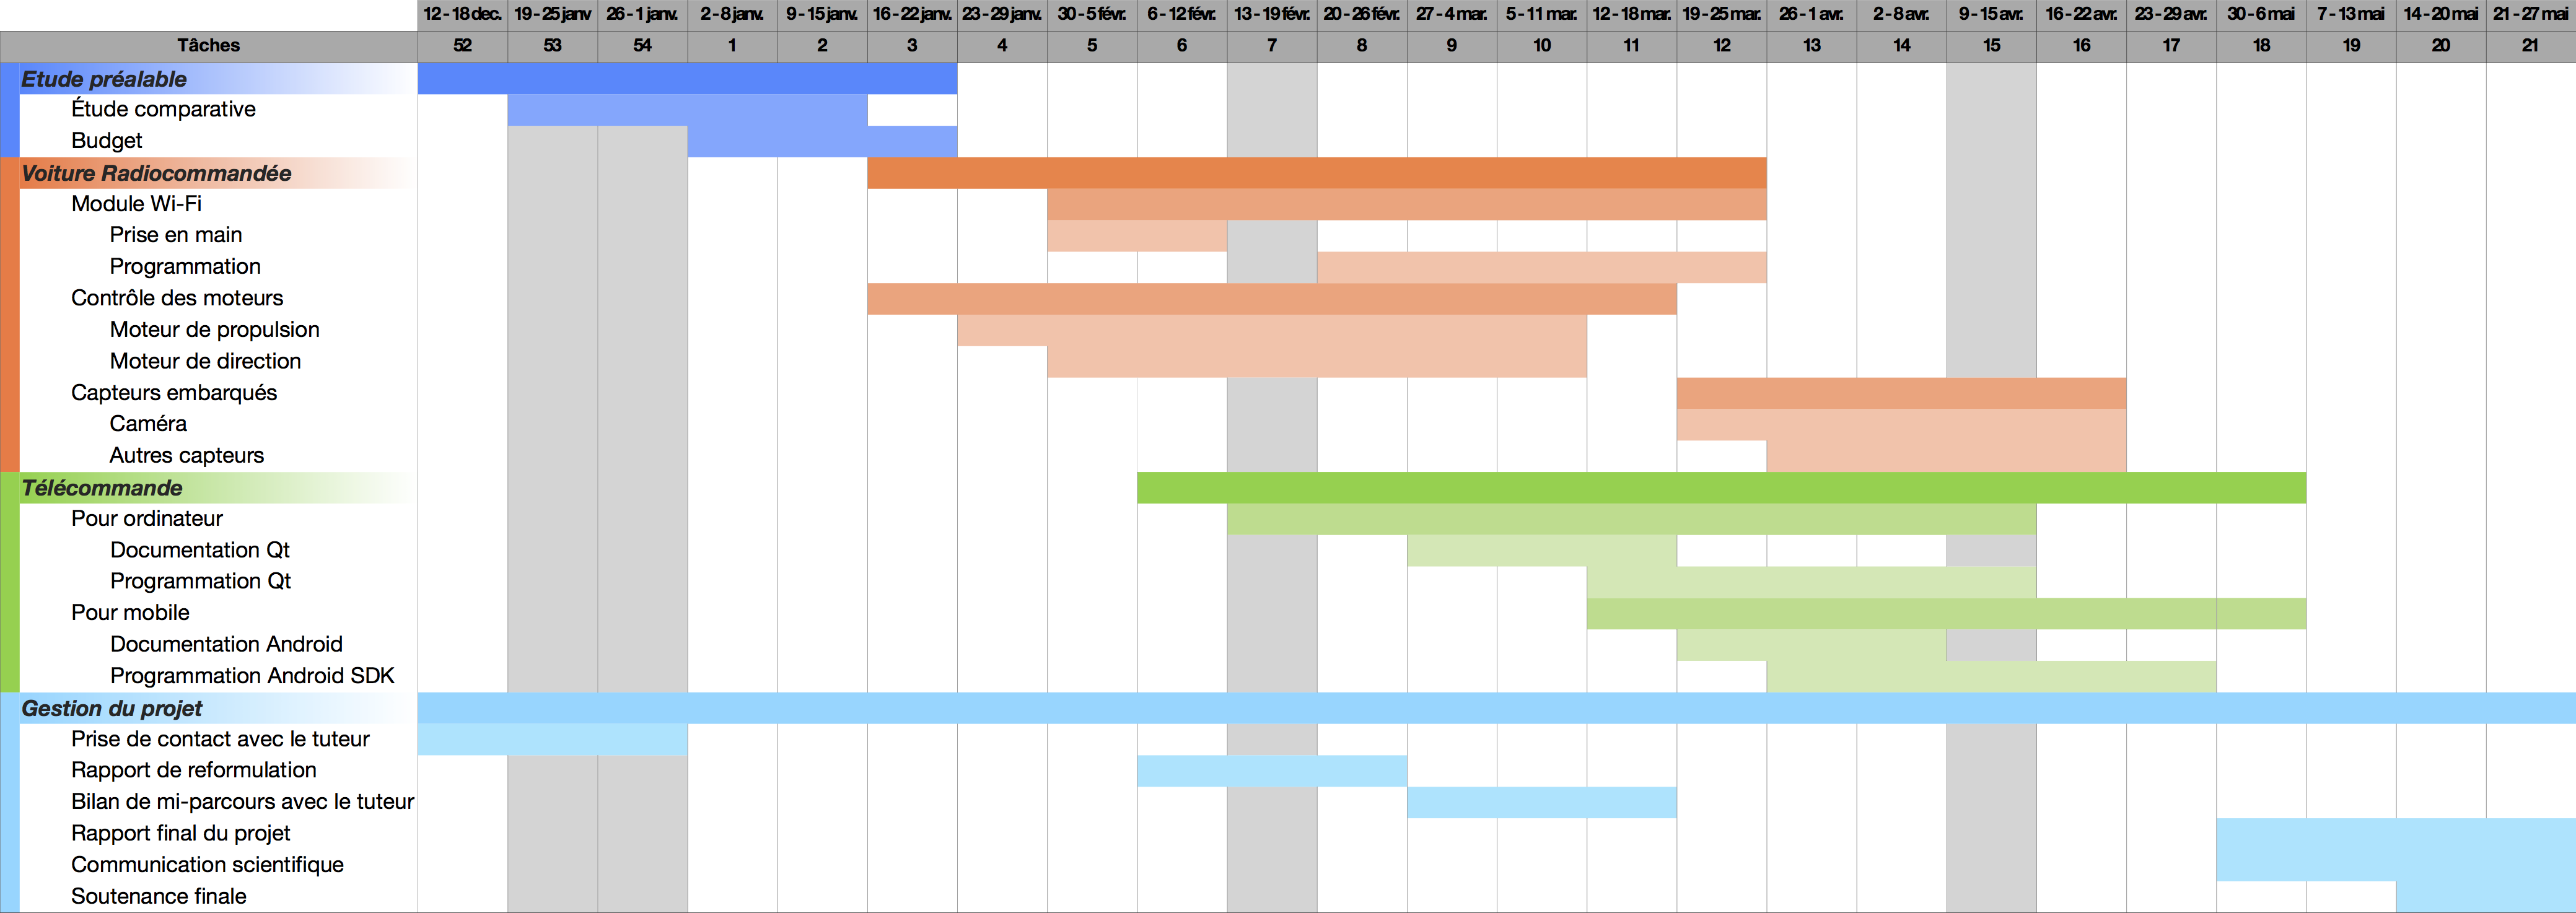
\includegraphics[scale=0.35, angle=90]{images/gantt.png}

\end{document}
